% ===============================================================
%  Postgraduate thesis template
%  Always check the latest formatting guidelines from your faculty
%  or the Institute for Postgraduate Studies, and adjust margins,
%  spacing and the title page to match.
% ===============================================================
\documentclass[12pt,a4paper,oneside]{report}

% ----- Layout -----
\usepackage[utf8]{inputenc}
\usepackage[T1]{fontenc}
\usepackage{lmodern}
\usepackage[left=4cm, right=2.5cm, top=2.5cm, bottom=2.5cm]{geometry}
\usepackage{setspace}
\onehalfspacing

% ----- Content -----
\usepackage{amsmath, amssymb, amsthm}
\usepackage{graphicx}
\graphicspath{{figures/}}
\usepackage{booktabs}
\usepackage{caption}
\usepackage{float}
\usepackage{enumitem}
\usepackage{xcolor}
\usepackage[nottoc]{tocbibind}

% ----- References -----
\usepackage[backend=biber, style=authoryear, maxcitenames=2, uniquename=false]{biblatex}
\addbibresource{references.bib}

\usepackage{hyperref}
\hypersetup{colorlinks=true, linkcolor=black, citecolor=teal, urlcolor=blue}

% ----- Theorems -----
\newtheorem{definition}{Definition}[chapter]
\newtheorem{theorem}{Theorem}[chapter]

% ----- Thesis details (used on the title page) -----
\newcommand{\thesistitle}{The Title of Your Thesis Goes Here}
\newcommand{\thesisauthor}{Your Full Name}
\newcommand{\thesisdegree}{Doctor of Philosophy}
\newcommand{\thesisfaculty}{Faculty of Computing and Informatics}
\newcommand{\thesisuniversity}{Multimedia University}
\newcommand{\thesisyear}{2026}

\begin{document}

% ---------------- Front matter ----------------
\pagenumbering{roman}
\begin{titlepage}
    \centering
    \vspace*{1cm}
    {\Large\bfseries\MakeUppercase{\thesistitle}\par}
    \vspace{3cm}
    {\large\MakeUppercase{\thesisauthor}\par}
    \vfill
    {\large\MakeUppercase{\thesisuniversity}\par}
    \vspace{0.5cm}
    {\large\thesisyear\par}
\end{titlepage}

\begin{titlepage}
    \centering
    \vspace*{1cm}
    {\Large\bfseries\MakeUppercase{\thesistitle}\par}
    \vspace{3cm}
    {\large BY\par}
    \vspace{0.5cm}
    {\large\MakeUppercase{\thesisauthor}\par}
    \vspace{3cm}
    {\large THESIS SUBMITTED IN FULFILMENT OF THE\\
    REQUIREMENTS FOR THE DEGREE OF\\
    \MakeUppercase{\thesisdegree}\par}
    \vspace{2cm}
    {\large (by Research)\par}
    \vfill
    {\large\MakeUppercase{\thesisfaculty}\\[0.3cm]
    \MakeUppercase{\thesisuniversity}\par}
    \vspace{0.5cm}
    {\large\thesisyear\par}
\end{titlepage}

\chapter*{Declaration}
\addcontentsline{toc}{chapter}{Declaration}

I hereby declare that the work has been done by myself and no portion of the work contained in this thesis has been submitted in support of any application for any other degree or qualification of this or any other university or institute of learning.

\vspace{2cm}

\noindent\rule{6cm}{0.4pt}\\
\thesisauthor\\
Date:

\chapter*{Acknowledgements}
\addcontentsline{toc}{chapter}{Acknowledgements}

I would like to thank my supervisor for their guidance and support throughout this research. I am also grateful to my family, friends and colleagues for their encouragement.

\chapter*{Abstract}
\addcontentsline{toc}{chapter}{Abstract}

Write a single-page summary of the thesis. State the research problem, the objectives, the methodology, the key findings and the contributions of the work. Avoid citations and abbreviations in the abstract.


\tableofcontents
\listoffigures
\listoftables
\chapter*{List of Abbreviations}
\addcontentsline{toc}{chapter}{List of Abbreviations}

\begin{tabular}{@{}p{3cm}l@{}}
    AI  & Artificial Intelligence \\
    CNN & Convolutional Neural Network \\
    MMU & Multimedia University \\
\end{tabular}


% ---------------- Main matter ----------------
\clearpage
\pagenumbering{arabic}
\chapter{Introduction}
\label{chap:intro}

\section{Background of the Study}
Introduce the research area and explain why it matters. Support your statements with references, for example \textcite{creswell2018} or \parencite{kothari2004}.

\section{Problem Statement}
Clearly state the problem this thesis addresses.

\section{Research Objectives}
The objectives of this research are:
\begin{enumerate}[label=\arabic*.]
    \item To investigate \ldots
    \item To develop \ldots
    \item To evaluate \ldots
\end{enumerate}

\section{Research Questions}
\begin{enumerate}[label=RQ\arabic*.]
    \item What \ldots?
    \item How \ldots?
\end{enumerate}

\section{Scope of the Study}
Describe what is included and excluded.

\section{Significance of the Study}
Explain the expected contributions.

\section{Thesis Organisation}
Chapter~\ref{chap:literature} reviews related work. Chapter~\ref{chap:method} describes the methodology. Chapter~\ref{chap:results} presents the results, and Chapter~\ref{chap:conclusion} concludes the thesis.

\chapter{Literature Review}
\label{chap:literature}

\section{Introduction}
Give an overview of the themes covered in this chapter.

\section{Theoretical Framework}
Discuss the theories that underpin the study \parencite{creswell2018}.

\begin{definition}
A \emph{definition} environment is available for formal terms.
\end{definition}

\section{Related Work}
Summarise and critique previous studies. Table~\ref{tab:related} compares them.

\begin{table}[H]
    \centering
    \caption{Summary of related studies.}
    \label{tab:related}
    \begin{tabular}{llp{6cm}}
        \toprule
        Study & Year & Key contribution \\
        \midrule
        \textcite{kothari2004} & 2004 & Research methodology fundamentals \\
        \textcite{creswell2018} & 2018 & Mixed-methods research design \\
        \bottomrule
    \end{tabular}
\end{table}

\section{Research Gap}
Identify what is missing in the literature and how this thesis addresses it.

\chapter{Methodology}
\label{chap:method}

\section{Research Design}
Describe the overall design of the study. Figure~\ref{fig:framework} shows the research framework.

\begin{figure}[H]
    \centering
    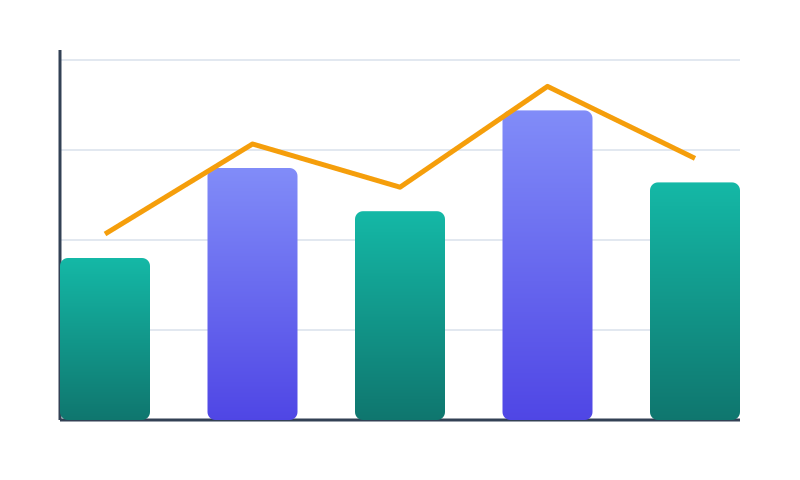
\includegraphics[width=0.65\textwidth]{sample-chart.png}
    \caption{Research framework (replace with your own figure).}
    \label{fig:framework}
\end{figure}

\section{Data Collection}
Explain how data were collected.

\section{Analysis}
Explain the analysis. For example, the mean is defined as
\begin{equation}
    \bar{x} = \frac{1}{n} \sum_{i=1}^{n} x_i .
    \label{eq:mean}
\end{equation}

\section{Ethical Considerations}
Describe ethical approval and consent procedures.

\chapter{Results and Discussion}
\label{chap:results}

\section{Results}
Present the findings in a logical order, using tables and figures.

\section{Discussion}
Interpret the results, relate them to the research questions and compare them with previous studies.

\chapter{Conclusion and Future Work}
\label{chap:conclusion}

\section{Summary of Findings}
Summarise how each objective was achieved.

\section{Contributions}
List the main contributions of this thesis.

\section{Limitations}
Acknowledge the limitations of the study.

\section{Future Work}
Suggest directions for future research.


% ---------------- References ----------------
\printbibliography[heading=bibintoc, title={References}]

% ---------------- Appendices ----------------
\appendix
\chapter{Supplementary Material}
\label{app:a}

Place questionnaires, extra tables, proofs or code listings here.


\end{document}
